\documentclass[a4paper]{article}
\usepackage[utf8]{inputenc}
\usepackage{fullpage}
\usepackage{biblatex}
\bibliography{expose.bib}
\usepackage{graphicx}
\title{Concept for a game prototype}
\author{Willi Schönborn}
\date{\today}
\begin{document}
\maketitle

\section*{Introduction}
The course \textit{Computer Graphics and Effects} (summer term 2011) at the \textit{Beuth Hochschule für Technik Berlin} contains a project assignment to build a game prototype using the jVR rendering framework. The purpose of this document is to explain the ideas and concepts for that game prototype.

\section*{Game Adaptation}
The idea is a partial port of a 2D arcade space shooter game available for mobile devices. The game is called PewPew and is currently available for free for the iPhone and Android platforms.

\begin{figure}[htbp]
\centering
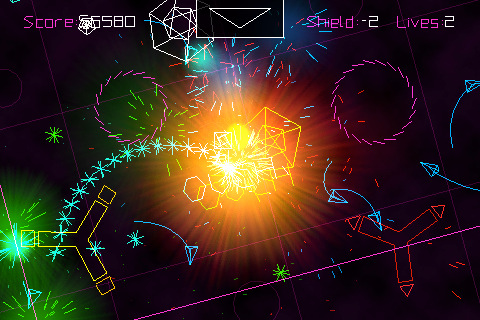
\includegraphics[width=0.7\textwidth]{PewPew-iPhone-App-Review.jpg}
\caption{Visual appearance}
\end{figure}

PewPew ships with several different game modes, levels and enemy types. The core game concept is extremely simple though: The Player has two virtual joysticks which can be used to control the movement of the ship and the direction of the fire. Despite the fact that the game has several game modes, it usually boils down to avoiding collisions and destroying enemies with the ship's gun. The game uses extremely simple vector and wireframe graphics extensively with the effect of a very harmonious visual appearance.

\newpage

\section*{Ideas and goals}
The main idea behind the game prototype is moving from flat 2D graphics to full 3D models while trying to preserve the overall look and feel of the game. To separate desired goals from optional or even undesired ones the next few paragraphs explain in detail which features are planned to be met and why.

\subsection*{Mandatory criteria}
All goals and ideas described as mandatory form the very basic goal of the prototype. Achieving these is the top priority. For complexity and time planning reasons the prototype will be limited to one game mode taking place in a single level. There will be one main ship, keyboard controls for movement and gun fire, at least one kind of enemies and collision detection. Hits and collisions should cause simple explosions. All objects participating in the game will have a self glowing effect. To emphasize the effect of speed fast moving particles should cause a blur effect.

\begin{figure}[htbp]
\centering
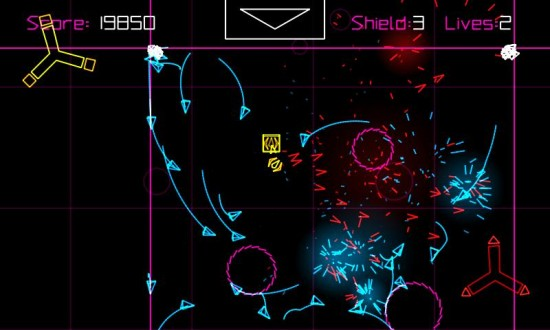
\includegraphics[width=0.7\textwidth]{4dd9c__pewpew-for-android-550x330.jpg}
\caption{Pandemonium game mode}
\end{figure}

\subsection*{Advisable criteria}
Everything named in this paragraph can be considered important for prototype to be considered complete but is not top priority. All these features will not be targeted even if there is only one mandatory criterion left to be implemented. Advisable criteria include a head-up-display which shows the current game score, the amount of shields and remaining lives. In addition to keyboard controls an integration with the Jinput library is planned to support a game controller with dual analog sticks, maybe even including force feedback.
shield, lives, score, game controller, dual analog sticks, force feedback, adjustable camera perspective

\subsection*{Optional criteria}
There are several features which would enhance the prototype but not very likely to be implemented. This includes a second gun fire mode, more advanced explosions, additional kinds of enemies and a split-screen style multiplayer mode allowing two players with gamepads playing at the same system.

\subsection*{Demarcation criteria}
To keep the prototype limited and the work load to an acceptable level some features will not be targeted by the prototype. Traditional light sources including shadows of any kind do not fit well in a wireframe style space arcade scenario and will therefore not be implemented. Neither will multiple levels, game modes nor a ranking of any kind be part of the prototype.

\newpage

\nocite{pewpewgame}
\nocite{iphoneappcafe}
\nocite{androidear}
\nocite{jinput}
\printbibliography

\listoffigures

\end{document}

